% !TeX root = ../libro.tex
% !TeX encoding = utf8

\chapter{Introducción}  \label{ch:Introduccion_informatica}

\noindent La tecnología se encuentra presente en prácticamente todas las tareas y disciplinas. Particularmente, en los últimos años hemos podido ver cómo el desarrollo de la \textbf{Inteligencia Artificial} ha permitido que tareas que antes se consideraban lentas o complicadas puedan realizarse rápidamente y con precisión con ayuda de un ordenador. En cambio, hay otras que todavía resultan complicadas de resolver de forma rápida tanto para expertos en la materia como para ordenadores. Es dentro de este conjunto dónde se va a desarrollar el presente trabajo, pues como veremos a continuación y en posteriores secciones apenas hay publicaciones relacionadas con el tema. En particular se desarrollará en el ámbito de las ciencias forenses, que explicaremos a continuación.

\medskip

\noindent Las \textbf{ciencias forenses} son aquellas que aplican el método científico a hechos presuntamente delictivos con la finalidad de aportar pruebas a efectos judiciales. Dentro de este campo destacan principalmente dos disciplinas: 

\begin{itemize}
    \item La \textbf{Criminalística}: disciplina encargada del descubrimiento y verificación científica de presuntos hechos delictivos y quienes los cometen.
    \item La \textbf{Medicina Forense}: disciplina encargada de determinar el origen de las lesiones, las caisas de muerte o la identificación de seres humanos vivos o muertos.
\end{itemize}

\medskip

\noindent Dentro de la medicina forense se encuentra la \textbf{antropología forense}, que principalmente se encarga de la identificación de personas a partir de restos óseos. Y es en este ambiente dónde se encuentra el proceso que da sentido a este trabajo.


\section{Descripción del problema}

\noindent Los antropólogos forenses emplean diversas técnicas para la identificación de personas a partir de restos óseos como son la reconstrucción de huesos, el cotejo fotográfico con el cráneo o el análisis de imágenes. De entre estas técnicas, destaca la \textbf{Superposición Craneofacial} por ser la que se encuentra más relacionada con el fin de este trabajo. Se trata de una técnica de identificación forense mediante la cual se comparan imágenes de la persona difunta (imágenes se le denominan imágenes ante-mortem) con una representación 3D de un cráneo candidato, con el fin de determinar si el cráneo pertenece a la persona de las imágenes o no. Se distinguen cuatro etapas en el proceso: 

\begin{enumerate}
    \item \textbf{Se recogen todas las imágenes y datos disponibles} de los sujetos ante-mortem, se realiza un escaneo $3D$ de los cráneos candidatos y se realiza el marcado de \textit{landmarks} o puntos de referencia. 
    
    \medskip
    
    \noindent El marcado de landmarks se realiza \textbf{de acuerdo a correspondencias morfológicas} tanto en la cara del sujeto en las imágenes como en el modelo $3D$ del cráneo candidato, de manera que cada punto marcado sobre el rosto tiene un homólogo marcado sobre el cráneo. Estos puntos de referencia reciben el nombre de \textbf{puntos craneométricos} cuando se marcan sobre el cráneo y \textbf{puntos cefalométricos} cuando se marcan sobre el rostro.
    \item \textbf{Análisis morfológico y morfométrico}: en esta etapa se realiza la selección de parejas imagen modelo $3D$ sobre las que realizar la superposición craneofacial.
    \item \textbf{Se realiza la superposición cráneo-cara} por parte del experto con ayuda de alguna herramienta como puede ser photoshop tratando de hacer corresponder cada landmark cefalométrico con su homólogo craneométrico.
    \item Se realiza la toma de decisiones en función de la bondad de los ajustes realizados.
\end{enumerate}

\begin{figure}[!h]
    \centering
    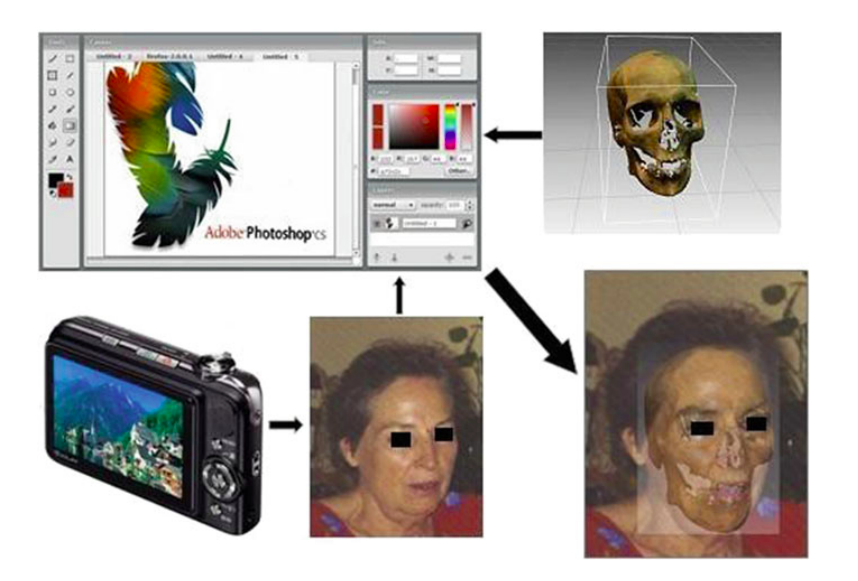
\includegraphics[width=0.8\textwidth]{img/ejemplo_SCF_intro.png}
    \caption{Ejemplo del proceso a seguir por el antropólogo forense en la superposición cráneo facial. Imagen extraida de \cite{damas2020handbook}.}
\end{figure}

\medskip

\noindent Sin embargo, esta tarea no es sencilla por factores diversos a tener en cuenta como son la grasa, la calidad de la imagen y el tejido blando facial que separa el punto craneométrico de su homólogo cefalométrico y que se traduce en una ligera traslación del punto. El desplazamiento ocasionado por el tejido blando facial no es constante ni se produce siempre en la misma dirección. Estos problemas, ocasionan que el experto forense tarde mucho en la tarea del marcado de landmarks. Una vez determinados los landmarks, un algoritmo automático puede encargarse de realziar el solapamiento del cráneo 3D y la imagen 2D acelerando el proceso y ahorrando tiempo en esta tarea al experto.

\begin{figure}[!h]
    \centering
    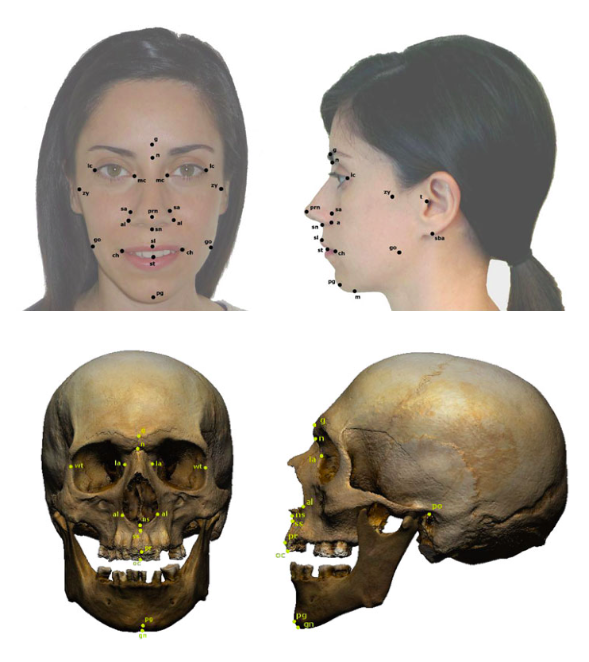
\includegraphics[width=0.9\textwidth]{img/marcado_landmarks.png}
    \caption{En esta imagen podemos ver la correspondencia entre landmarks craneométricos y cefalométricos. Algunos de los landmarks que aparecen en la imagen serán estudiados en este trabajo. Imagen extraida de \cite{damas2020handbook}.}
\end{figure}


\newpage

\noindent En este trabajo se estudiarán un total de $30$ landmarks, que son los siguientes: 

\begin{center}
    \begin{tabular}{ |c|l|l|c| } 
        \hline
         & \textbf{Landmarks} & \textbf{Notación} \\
        \hline
        1 & Menton & Me \\ 
        2 & Gnathion & Gn \\ 
        3 & Pogonion & Pg \\ 
        4 & Prosthion & Pr \\ 
        5 & Labiale Superius & Ls \\ 
        6 & Subnasale & Sn \\ 
        7 & Nasion & N \\ 
        8 & Glabella & G’ \\ 
        9 & Vertex & v \\ 
        10 & Left Gonion & GoL \\ 
        11 & Right Gonion & GoR\\ 
        12 & Left Zygion & zyL \\ 
        13 & Right Zygion & zyR\\ 
        14 & Left Alare & alL \\ 
        15 & Right Alare & alR \\ 
        16 & Left Endocanthion & EnL \\ 
        17 & Right Endocanthion & EnR \\ 
        18 & Left Exocanthion & ExL \\ 
        19 & Right Exocanthion & ExR \\ 
        20 & Left Tragion & T’L \\ 
        21 & Right Tragion & T’R \\ 
        22 & Infradentale & Id \\ 
        23 & Trichion & Tr \\ 
        24 & Supramentale & sm\\ 
        25 & Left Frontotemporale & FtL \\ 
        26 & Right Frontotemporale & FtR \\ 
        27 & Left Frontozygomaticus & fzL \\ 
        28 & Right Frontozygomaticus & fxR \\ 
        29 & Left Midsurpaorbital & msoL \\ 
        30 & Right Midsupraorbital & msoR \\ 
        \hline
    \end{tabular}
\end{center}

\medskip 


\section{Motivación}

Actualmente, este proceso del marcado de landmarks es costoso y complicado de replicar, y pese a los avances actuales que se están llevando a cabo para automatizar esta tarea \cite{Huete2015PastPA}, la identificación de \textit{landmarks} sigue realizándose a mano normalmente. Sin embargo en la identificación de landmarks \textbf{craneométricos} podemos encontrar algunos trabajos publicados como \cite{bermejo2021automatic} que permiten una atomatización de esta parte del proceso. En este contexto, el presente trabajo tratará de proporcionar una solución automática al proceso del marcado de \textbf{landmarks cefalométricos} (en imágenes ante-mortem).

\medskip

\noindent El algoritmo que buscamos debería tener unos requisitos mínimos: 

\begin{itemize}
    \item Debe ser un método \textbf{robusto}, en el sentido de que debe abarcar todos los posibles casos y variaciones del problema. En nuestro caso se traduce en saber lidiar con imágenes frontales, de perfil o $3/4$ junto con otros factores como la calidad de la imagen, iluminación y oclusiones parciales. En todos los casos anteriores, el algoritmo debería tener un buen comportamiento.
    \item Capaz de operar con un \textbf{pequeño conjunto de datos}, ya que como hemos comentado anteriormente, se dispone generalmente de pocas imágenes para realizar el marcado de landmarks.
    
    \medskip

    \noindent Esta propiedad es deseable porque generalmente, en los problemas forenses reales, no se dispone de una amplia variedad de imágenes de la persona desaparecida, en algunos casos sólo se dispone de unas pocas imágenes y no todas van a ser frontales y con buena calidad e iluminación.

    \item Debe proporcionar siempre una solución lo más \textbf{correcta} posible.  
    
    \item Debe ser \textbf{eficaz} y \textbf{eficiente}. Buscamos acelerar el proceso del marcado de landmarks considerablemente a la par que conseguir resolver el objetivo principal.
\end{itemize}

\noindent Remarcamos que la intención no es reemplazar al experto en su labor del marcado de landmarks sino proporcionar una ayuda para acelerar el proceso.

\medskip 

\noindent Debido a que el algoritmo va a operar con imágenes, buscamos una solución dentro del área de la \textbf{visión por computador}. Actualmente existen  multitud de trabajos relacionados con el marcado de landmarks en imágenes dentro de este área, la mayoría usando algoritmos de \textbf{deep learning} y enfocadas al reconocimiento de individuos en imágenes. Los landmarks que marcan en estas propuestas no siguen correspondencias morfológicas, y dependen únicamente de la estructura facial del individuo. Dichos algoritmos son entrenados con grandes bases de datos de imágenes etiquetadas y actualmente se obtienen excelentes resultados en este tipo de problemas. En particular nos hemos fijado en el framework \textbf{3FabRec}\cite{browatzki20203fabrec}.Dicho framework cuenta con excelentes resultados en la tarea de detección de landmarks en imágenes y sobre todo nos interesa porque obtiene buenos resultados entrenando con pocas imágenes. Es este artículo el que supone el punto de partida para este trabajo, debido a que nos parece una buena alternativa tratar de adaptar este framework a la detección de landmarks cefalométricos en imágenes usando un dataset forense que contiene pocas imágenes etiquetadas por un experto.

\section{Objetivos}

\noindent Los objetivos a resolver en el trabajo son los siguientes: 

\begin{enumerate}
    \item Realizar una investigación sobre el estado del arte en la localización de landmarks cefalométricos en fotografías en el ámbito de la antropología forense.
    \item Afianzar conocimientos adquiridos sobre Aprendizaje Automático y Visión por computador.
    \item Realizar una investigación sobre los modelos de Auteoncoders y redes Adversarias existentes.
    \item Realizar un estudio en el dataset proporcionado para identificar errores o anomalías.
    \item Generar un nuevo dataset a partir del proporcionado realizando un cropping de las imágenes originales para quedarnos únicamente con la cara del sujeto y poder entrenar la red.
    \item Realizar un estudio experimental realizando diversas pruebas sobre el framework con el conjunto de datos proporcionado.
\end{enumerate}

\section{Planificación}
    \noindent La planificación del proyecto desde un comienzo fue pensada para llevar a cabo el desarrollo del software siguiendo un modelo en cascada, un modelo que evita la vuelta atrás entre etapas. Sin embargo, debido a que el desarrollo consistirá principalmente en una adaptación de un software ya existente a un problema concreto, se estimó desde un principio que en esta etapa no se desarrollaría un programa de gran complejidad, sabíamos que el software podría sufrir ligeras modificaciones en función de los resultados obtenidos durante la experimentación, es por ello que se optó por un modelo de ciclo de vida en cascada retroalimentado como se puede ver en \autoref{Fig::Ciclo de vida}:


    \begin{figure}[!h]
        \centering
        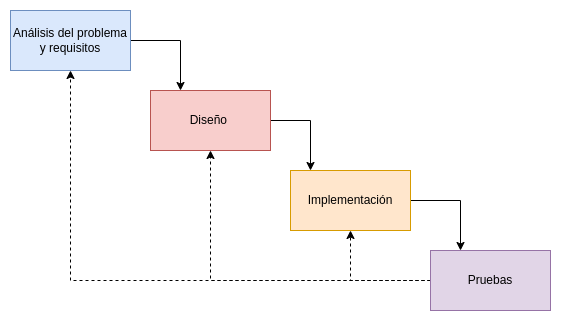
\includegraphics[width=0.8\textwidth]{img/disenio_cascada.png}
        \caption{Diseño en cascada retroalimentado empleado.}
        \label{Fig::Ciclo de vida}
    \end{figure}

    \medskip

    \noindent Las etapas que se seguirán serán las siguientes:

    \begin{enumerate}
        \item \textbf{Análisis del problema y requisitos}: En esta tapa se profundizará sobre el contexto y la importancia del problema a resolver y se llevarán a cabo reuniones con los tutores del trabajo para aclarar los requisitos y objetivos concreto del software a desarrollar. 
        \item \textbf{Diseño}: En nuestro caso, en esta etapa se realizarán dos tareas: 
        
        En primer lugar se diseñará el estudio de la base de datos que emplearemos así como las transformaciones que deban sufrir los datos para poder ser empleados por el software que emplearemos en la fase de experimentación. 

        En segundo lugar se diseñarán los experimentos a realizar así como las técnicas que se aplicarán, las métricas y los protocolos de validación que se usarán.

        \item \textbf{Implementación}: Se implementan todas las técnicas diseñadas en la etapa anterior.
        \item \textbf{Experimentación}: Se ponen en práctica todos los experimentos diseñados de forma teórica y se obtienen resultados. En función de estos se valora una vuelta atrás en el ciclo de vida del software para realizar modificaciones en el software.
    \end{enumerate}
    
    \medskip

    \noindent Debido a la alta carga de trabajo durante el curso, desde un comienzo, el desarrollo del trabajo se planificó pensando en su defensa para la convocatoria extraordinaria de Septiembre o para la convocatoria especial de Noviembre. Por ello, la planificación original por meses se puede observar en la \autoref{Fig::Planificacion original}.


    \begin{figure}[!h]
        \centering
        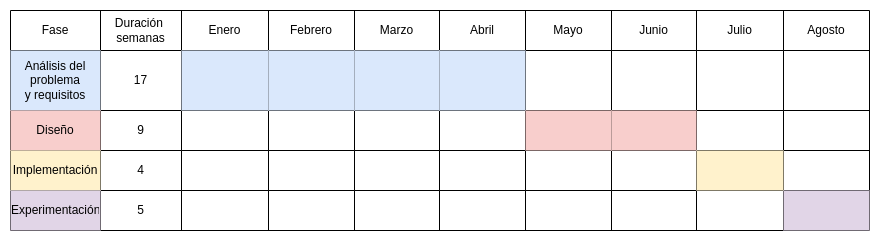
\includegraphics[width=0.9\textwidth]{img/plan_provisional.png}
        \caption{Planificación original.}
        \label{Fig::Planificacion original}
    \end{figure}

    \medskip

    \noindent Dentro de la semana computan únicamente los días de Lunes a Viernes. Resalta a la vista la gran cantidad de semanas invertidas en las primeras dos etapas con respecto a las invertidas en las dos últimas. El principal motivo para repartir el tiempo de esta manera es que durante el curso se calculó que sería imposible dedicar al trabajo más de \textbf{cuatro horas por semana}. En cambio, una vez terminado el curso se previó dedicar una media de \textbf{seis horas diarias al trabajo}. Es por ello que a pesar de la gran diferencia de semanas, si miramos las horas obtenemos:
    
    \begin{itemize}
        \item Para la primera fase se invirtieron un total de \textbf{68 horas}.
        \item Para la segunda fase un total de \textbf{36 horas}.
        \item Para la tercera y cuarta fase se invirtieron un total de \textbf{120 horas} para cada una.
        \item En total el tiempo estimado de desarrollo del proyecto fue de \textbf{344 horas}.
    \end{itemize}
        
    \noindent No obstante, esta estimación resultó ser muy ajustada para completar el trabajo, lo que ocasionó que se retrasara la entrega del mismo a Noviembre, es por ello que el plan definitivo del proyecto se puede ver en la \autoref{Fig::Planificacion final}. Aquí se puede ver cómo desde Septiembre, a causa de los resultados obtenidos en la experimentación, se vuelve atrás en el ciclo de vida del software a la parte de análisis del problema y requisitos para consultar a los tutores con los resultados obtenidos y modificar el resto de etapas sucesivas. El tiempo invertido por día en esta segunda fase fue de \textbf{4 horas} diarias. Lo que incrementa el tiempo total invertido a:

    \begin{itemize}
        \item \textbf{148 horas} para la primera fase.
        \item Para la segunda fase un total de \textbf{76 horas}.
        \item Para la tercera y cuarta fase se invirtieron un total de \textbf{160 horas} para cada una.
        \item En total el tiempo estimado de desarrollo del proyecto fue de \textbf{544 horas}.
    \end{itemize}

    \begin{figure}[!h]
        \centering
        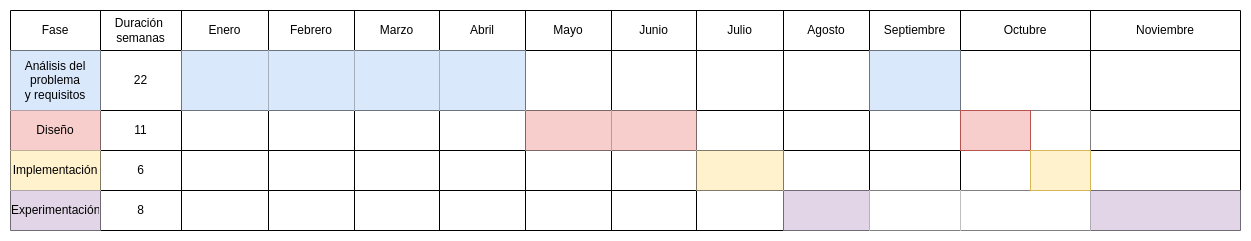
\includegraphics[width=0.95\textwidth]{img/plan_definitivo.png}
        \caption{Planificación original.}
        \label{Fig::Planificacion final}
    \end{figure}

    \medskip

    \noindent Como consecuencia, en un principio se preveía usar un total de \textbf{344} horas para finalizar el trabajo, pero finalmente hicieron falta \textbf{544} horas, de esta forma, si se supone que un Investigador en una empresa de base tecnológica es de 35€/hora, a partir de los resultados obtenidos, el trabajo tenía un presupuesto inicial de \textbf{12.040 €} que finalmente fue ampliado a \textbf{19.040 €}.

\endinput
%------------------------------------------------------------------------------------
% FIN DEL CAPÍTULO. 
%------------------------------------------------------------------------------------


